\documentclass[letterpaper,11pt]{article}
\usepackage{amsmath, amsthm, amssymb}
\usepackage{bridges}
\usepackage{graphicx}

\usepackage[colorlinks=true, urlcolor=blue, citecolor=black, linkcolor=black]{hyperref}
\usepackage{subcaption}

\usepackage{algorithm}
\usepackage{algpseudocode}
\usepackage{hyperref}

%\usepackage{svg}
\usepackage{multirow}
\usepackage{caption}
\usepackage{tikz}
\usepackage{transparent}

\usepackage[bottom]{footmisc}

\urlstyle{rm}

\sloppy
\usepackage{listings}
\lstset{breaklines=true}

\title{ A Generalized 2D and 3D Hilbert Curve }
\author{ Jakub \v{C}erven\'{y} and Zzyv Zzyzek }

\date{}

\begin{document}

\maketitle

\begin{abstract}
  The two and three dimensional Hilbert curves are fractal space filling curves that
  map the unit interval to the unit square or unit cube while preserving a notion
  of closeness, or locality, after the map.
  We present the Gilbert curve,
  a conceptually straight forward generalization of the Hilbert curve,
  that works on arbitrary rectangular regions, overcoming the limitation of the Hilbert
  curve that requires side lengths be exact powers of two.
  Our construction of the Gilbert curve provides a notion of \textit{harmony}
  that provide alternate subdivision schemes when a side length is much larger than the rest,
  creating more visual pleasing curves as a result.
\end{abstract}


\section*{Generalized Hilbert Curves}

In a website application and scanned note \cite{lutanho2003}, Tautenhahn provided the basis for a generalized 2D
space filling curve.
Tautenhahn also included policies for when to subdivide regions preferentially in only one dimension
that help to create more \textit{harmonious} curve realizations.
Tautenhahn's exploration details the parity arguments necessary for when a subdivision scheme can be employed
without creating diagonal moves, where diagonal moves are called \textit{notches} here.


In this paper, we extend Tautenhahn's ideas to create a 2D and 3D generalized Hilbert curve.
We further extend Tautenhahn's core ideas on when to use alternate subdivision schemes when one length is much
larger than the rest, what we call \textit{eccentric cases}, and apply them to a 3D generalized Hilbert curve.
Tautenhahn's unpublished reasoning behind the constants used in the 2D eccentric split case are briefly discussed
%later\footnote{Through personal communication with the authors, Tautenhahn kindly provided the reasoning for the constants used in the eccentric split}.
later\footnotemark[1].

%????
%The idea of generalizing Hilbert curves is not new and one notable 2D attempt was by Zhang, Kamata and Ueshige \ref{zhang2006}.
%Whereas their method works for arbitrary side lengths, the resulting curves tend to have runs of straight lines for non powers of two
%side lengths.
%Further their is complicated with no clear way to generalize it 3D.
%
%Anders used a Hilbert curve mapping to
%visualize the human genome as a 2D map \ref{anders2009}. Cortesi has
%used a Hilbert curve to visualize binary files \ref{cortesi2011}.
%
%For a more technical introduction to the space filling curves, including the Hiblert curve, the reader is refered to Sagan \ref{sagan1994}.
%

\footnotetext[1]{Through personal communication with the authors, Tautenhahn kindly provided the reasoning for the constants used in the eccentric split}.

\begin{figure}[!htb]

  \begin{minipage}{0.48\textwidth}

    \centering
    \includegraphics[width=\linewidth]{gilbert2d_examples.pdf}
    \caption{ 2D Gilbert curves for i) $8 \times 8$, ii) $18 \times 6$, iv) $13 \times 8$ (with notch), iv) $14 \times 14$ }
    \label{fig:gilbert2d_examples}
  \end{minipage}\hfill
  \begin{minipage}{0.48\textwidth}
    \centering
    \includegraphics[width=\linewidth]{gilbert3d_orig_examples.pdf}
    \caption{ 3D Gilbert curves for i) $4 \times 4 \times 4$, ii) $6 \times 6 \times 6$, iii) $8 \times 4 \times 4$, iv) $5 \times 4 \times 4$ (with notch) }
    \label{fig:examples3d}

  \end{minipage}

\end{figure}


\begin{figure}[!htb]

  \centering
  \includegraphics[width=\linewidth]{simple_hampath_flat.pdf}
  \caption{ Examples of Hamiltonian paths for small grid sizes. A red `x' corresponds to no possible path for the chosen endpoints. }
  \label{fig:exampleHampath}

\end{figure}


\section*{Valid Paths from Grid Parity}

%\begin{figure}[!htb]
%
%  \begin{minipage}{0.48\textwidth}
%
%    \centering
%    %\begin{table}[h]
%    %  \centering
%      \begin{tabular}[t]{cr|cc}
%        \multicolumn{2}{c}{ \multirow{2}{*}{Path Possible} } & \multicolumn{2}{c}{Volume} \\
%        & & \textit{even} & \textit{odd} \\
%        \hline
%          %\multirow{2}{*}{$|\alpha| \bmod 2$} & \textit{even} & Yes & Yes \\
%          \multirow{2}{*}{ $|\alpha|$ } & \textit{even} & Yes & Yes \\
%           & \textit{odd} & \textbf{No} & Yes \\
%         \hline
%      \end{tabular}
%      \caption{ $|\alpha|$ is the distance of endpoints.
%                A Hamiltonian path is possible only when $|\alpha|$ is even or both
%                $|\alpha|$ and the volume are odd. }
%      \label{table:pathTable}
%    %\end{table}
%
%  \end{minipage}\hfill
%  \begin{minipage}{0.48\textwidth}
%
%    \centering
%    \includegraphics[width=\linewidth]{simple_hampath.pdf}
%    \caption{ Examples of Hamiltonian paths for small grid sizes. A red `x' corresponds to no possible path for the chosen endpoints. }
%    \label{fig:exampleHampath}
%
%  \end{minipage}
%
%\end{figure}

The feasibility of determining whether there exists a non intersecting path, called a \textit{Hamiltonian path},
connecting endpoints on the corners in a rectangular cuboid
grid region can be accomplished through parity arguments.
Label grid cell points in a volume as 0 or 1,
alternating between labels with every axis-aligned single step move.
Any Hamiltonian path that ends at one of the three remaining corners has to have the same parity as the starting point if the
volume is odd, or different parity if the volume is even.

Figure \ref{fig:exampleHampath} illustrates this for starting position $(0,0)$ with areas $(2 \times 2)$, $(3 \times 2)$ and $(3 \times 3)$,
where a red cross indicating a precluded endpoint.
When a Hamiltonian path is not precluded by the parity of the start and end point, we say that the endpoints are \textit{color compatible}.
In general, color compatibility is a necessary, but insufficient, test for a Hamiltonicity.

In the simpler case when the region is a rectangular cuboid and endpoints are on the corners of the cuboid region, color compatibility
is a sufficient test for Hamiltonicity.
This allows us a simple test to see if there is a Hamiltonian path within a rectangular region purely based on the parity of side lengths
and the corner locations of the start and end points of the path.

For the constructed 2D and 3D Gilbert curves in this paper, we don't use endpoints that are diagonal within a cuboid region and
only use endpoints that are in line in a single axis-aligned direction.

%For a path starting at $(0,0,0)$ and ending $|\alpha|$ steps in one of the axis-aligned dimensions,
%then Table \ref{table:pathTable} enumerates this condition under which a valid path is possible.

%Assuming a curve starts from position $p_s=(0,0,0)$ and has proposed
%endpoint at $p_e=((w-1),0,0)$, with a cuboid region as $\alpha = (w,0,0), \beta = (0,h,0), \gamma = (0,0,d)$.

%We focus on optimizing for providing a notch-free path when all side lengths are even and allow notches when $|\alpha|$ is odd in 2D
%or when one of the side lengths is odd in 3D.

%The 2D Gilbert curve limits the number of notches to one.
%The 3D Gilbert curve's subdivision strategy creates a notch when the distance between endpoints is odd,
%potentially creating more than one notch.
%
%In both the 2D and 3D case, when the original side lengths are all even, no notches will be present.
%



\begin{figure}[!htb]

  \begin{minipage}{0.55\textwidth}

    \begin{minipage}{1.0\textwidth}
      \centering
      \includegraphics[width=\linewidth]{gilbert2d_mainsubdiv.pdf}
      \caption{ Subdivision template for the 2D Gilbert curve. }
      \label{fig:main2dsubdiv}
    \end{minipage}

    \begin{minipage}{1.0\textwidth}
      \centering
      \includegraphics[width=0.65\linewidth]{gilbert2d_example_mainsubdiv.pdf}
      \caption{ Example curve with subdivision regions highlighted. }
      \label{fig:main2dsubdivExample}
    \end{minipage}

  \end{minipage}\hfill
  \begin{minipage}{0.45\textwidth}
    \centering
    \includegraphics[width=\linewidth]{gilbert3d_explode.pdf}
    \caption{ The main subdivision template for the 3D Gilbert curve. }
    \label{fig:gilbert3DJSplit}
  \end{minipage}

\end{figure}

\section*{Subdivision Templates}

For both the 2D and 3D Gilbert curve, a subdivision template is chosen to recursively partition the region.
Figure \ref{fig:main2dsubdiv} shows the 2D template and figure \ref{fig:gilbert3DJSplit} shows the 3D template.
Figure \ref{fig:main2dsubdivExample} provides a 2D example of the main subdivision with regions labelled and color coded.

The vectors $\alpha, \beta, \gamma \in \mathbb{Z}^3$ provide generalized notions of width ($\alpha$), height ($\beta$),
and depth ($\gamma$), so that we can transform rectangular or cuboid regions as necessary for the recursion.
Each of $\alpha, \beta, \gamma$ will only have one non-zero component and will be orthogonal to each other,
representing a snapshot of the current frame of reference.

When dividing into sub-regions, side lengths are chosen to be integral.
Even side lengths are preferred for the first subdivided region (region \textit{A} in figures \ref{fig:main2dsubdiv} and \ref{fig:gilbert3DJSplit}).
A path is recursively chosen for each of the sub-regions and, after resolution, endpoints are connected.
Figure \ref{fig:production2d} shows the choice in 2D of even or odd regions depending on side length parity.

When regions have a side length that is much larger than the rest, another subdivision scheme is used.
We call these cases \textit{eccentric subdivisions}, as the larger side length makes the
region lopsided.

The eccentric subdivision schemes provide a more visually pleasing partition of the space, as regimented subdivisions might take paths
that are long and skinny or wide and squat.
In the next section,
We will briefly go over motivations for the threshold values for the 2D eccentric subdivision scheme in the next section
but first provide a more detailed desciption of the template subdivision schemes for the 2D and 3D Gilbert curve below.

\subsection*{2D Gilbert Curve}

For the 2D Gilbert curve,
if the width like dimension ($\alpha$) is much larger, the curve is split in half along
the $\alpha$ length (figure \ref{fig:eccentric_2d_alg}, \ref{fig:eccentric_2d_example_alg}).
If no eccentric split is done, the region is subdivided into two squares at the bottom and a rectangle on top, with endpoints
joined on the outer perimeter.

Each regions parity is chosen so as to try to keep color compatibility, ensuring a valid path if possible.
When the side lengths are exact powers of two, the resulting curve is identical to the 2D Hilbert curve.

If the region is odd parity, with both side lengths odd, a notch is forced and is directed to the upper right region,
as illustrated by figure \ref{fig:production2d}.

\subsection*{3D Gilbert Curve}

In the normal case, a subdivision scheme is used to split the cuboid into five regions, two
cube like regions where the path starts and stops, and three oblong cuboid regions for the middle portion of the path.
Figure \ref{fig:gilbert3DJSplit} provides an exploded view of the main subdivision and where the endpoints line up.
See also figure \ref{fig:gilbert3d_bulk_template} for the template and figure \ref{fig:gilbert3d_bulk_example}
for a $10 \times 10 \times 10$ example, with each region color coded.

Endpoints within a sub-divided region are kept on the exterior of the region and joined after the resulting recursion
has completed.
As with the 2D Gilbert, when side dimensions are equal and exact powers of two, the resulting curve is identical to the
corresponding 3D Hilbert curve.

Durcing the course of sub-division, if the width like dimension ($\alpha$) is much larger, the curve is split in half along
the $\alpha$ length (figure \ref{fig:gilbert3d_eccentric_alpha}, \ref{fig:gilbert3d_eccentric_alpha_example}).
If the $\alpha$ eccentric split is not triggered, the height-like dimension, $\beta$, is then compared to depth-like dimension, $\gamma$
and if very much larger, an eccentric subdivision scheme is used that splits in the $\alpha$ and $\beta$ direction
(figure \ref{fig:gilbert3d_eccentric_beta}, \ref{fig:gilbert3d_eccentric_beta_example}).
If both $\alpha$ and $\beta$ are not much larger, a check is done to see if the depth-like dimension, $\gamma$, is much larger than 
than the height-like dimension, $\beta$, splitting in the $\alpha$ and $\gamma$ direction if so
(figure \ref{fig:gilbert3d_eccentric_gamma}, \ref{fig:gilbert3d_eccentric_gamma_example}).

If any of the subdivided regions has endpoints that lay in a direction with
odd length, a notch will appear.
This means the number of notches for the 3D Gilbert curve isn't limited to one in the case a side length is odd.

\begin{figure}[!htb]
  \centering
  \includegraphics[width=\linewidth]{config_production.pdf}
  \caption{ Enumeration of the subdivision template depending on different parities of $\alpha$ and $\beta$ dimensions. }
  \label{fig:production2d}
\end{figure}

\section*{Eccentric Subdivision}

When side lengths become too lopsided, an alternate \textit{eccentric} subdivision scheme is chosen to split along
the larger side length.

For each eccentric subdivision, a proportion threshold needs to be chosen to determine when a side
lengths become too lopsided to warrant an alternate subdivision.
Here we motivate the eccentric subdivision constants for the 2D case.

Consider a \textit{defect} function, $\lambda _ 2 : \mathbb{N}^2 \mapsto \mathbb{N}$, that measures the area relative
to what the area would be if just the minimum side length were taken:

$$
\begin{array}{ll}
  \lambda _ 2 (|\alpha|,|\beta|) = \frac{ |\alpha| \cdot |\beta| }{ \text{min}(|\alpha|,|\beta|)^2 } \\
\end{array}
$$

If there is a disjoint subdivision of a volume $V_0$ to $V_1  = ( V _ {0,0}, V _ {0,1}, \dots, V _ {0,m-1} )$,
($V _ 0  = \cup _ {k} V _ {0,k}$),
define the subdivided volume's \textit{average defect} to be the sum of defects weighted by their proportional volume:

$$
\begin{array}{l}
  \lambda _ {s} ( V _ 1 ) = \sum _ {k} \frac{ \text{Vol}(V _ {0,k}) }{ \text{Vol}( V _ 0 ) } \cdot \lambda _ 2( V _ {0,k} )
\end{array}
$$

The defect gives a coarse idea of how lopsided or \textit{eccentric} a region is.
If the defect is too high, we might want to split the larger sides while keeping the smaller sides the same size.
Reducing the average defect attempts to make each subdivided region more square-like.
When subdivided areas are more square-like, we say that the subdivided regions are more \textit{harmonious}.

If the $\alpha$ side length is significantly longer than the $\beta$ side length,
we want to subdivide the rectangle into two nearly equal regions and recursively find
a Gilbert curve in each region.
We will justify the constant $(3/2)$ as the ratio threshold to split on, using an argument
originally developed by L. Tautenhahn \footnote{ Given to us through personal communication with L. Tautenhahn }.

The defect of a rectangle with side length $|\alpha|$ and $|\beta|$, assuming $|\alpha| > |\beta|$, is $(|\alpha| / |\beta|)$.
After subdivision, if we assume $|\alpha| < 2 |\beta|$, the resulting defect is $2 |\beta| / |\alpha|$.
For a defect reduction, we search for conditions in which the ratio of the resulting defect to the original defect is less than unity,
giving the equation $|\alpha| / |\beta| > \sqrt{2}$.

Since $\sqrt{2} \approx 1.4142 < (3/2)$, if we choose $|\alpha| / |\beta| > (3/2)$ we can
be assured a defect reduction.
In the case when $|\alpha| > 2 |\beta|$, it is easy to verify that the defect is always reduced
\footnote{ The ratio of the defects before and after the split is $(1/2)$ }.

Defect reductions for the 3D case can be done, but are more complicated.
The constants for the 3D subdivision in this paper were observed to yield visually pleasing results
without concern for optimizing defect reduction.


\begin{minipage}[!htb]{0.43\linewidth}
\begin{algorithm}[H]
  \caption{Gilbert 2D}
  \label{alg:gilbert2d}
  \begin{algorithmic}

    \State \textit{\# $p, \alpha, \beta \in \mathbb{Z}^3$}
    \Function{Gilbert2D}{$p$, $\alpha$, $\beta$}
      \State $\alpha_2, \beta_2  = \text{div}(\alpha, 2), \text{div}(\beta, 2)$
      \If{ $(|\beta| \equiv 1)$ }
        \State \textbf{yield} $p + i \cdot \delta(\alpha)$ \textbf{forall} $i \in |\alpha|$
      \ElsIf{ $(|\alpha| \equiv 1)$ }
        \State \textbf{yield} $p + i \cdot \delta(\alpha)$ \textbf{forall} $i \in |\beta|$
      \ElsIf{ $(2 |\alpha| > 3 |\beta|)$ }
        \If{ $(|\alpha_2| > 2)$ and \\ \hskip4.12em $(|\alpha_2| \bmod{2} \equiv 1)$ }
          \State $\alpha_2 \leftarrow \alpha_2 + \delta(\alpha)$
        \EndIf
        \State \textbf{yield} Gilbert2D($p$, $\alpha_2$, $\beta$)
        \State \textbf{yield} Gilbert2D($p + \alpha_2$, $\alpha - \alpha_2$, $\beta$)
      \Else
        \If{ $(|\beta_2| > 2)$ and \\ \hskip4.12em $(|\beta_2| \bmod{2} \equiv 1)$ }
          \State $\beta_2 \leftarrow \beta_2 + \delta(\beta)$
        \EndIf
        \State \textbf{yield} Gilbert2D($p$, \\ \hskip9.75em $\beta_2$, $\alpha_2$)
        \State \textbf{yield} Gilbert2D($p + \beta_2$, \\ \hskip9.75em $\alpha$, $(\beta - \beta_2)$)
        \State \textbf{yield} Gilbert2D($p + (\alpha - \delta(\alpha)) +$ \\ \hskip9.75em $(\beta_2 - \delta(\beta))$, \\ \hskip9.75em $\beta_2$, $-(\alpha - \alpha_2)$)
      \EndIf
    \EndFunction

  \end{algorithmic}
\end{algorithm}
\end{minipage}\hfill
\begin{minipage}[!htb]{0.43\linewidth}

  \begin{minipage}[ht]{0.49\linewidth}

    \centering
    \includegraphics[width=0.925\linewidth]{gilbert2d_eccentric_alpha1.pdf}
    \captionof{figure}{ }
    \label{fig:eccentric_2d_alg}

  \end{minipage}\hfill
  \begin{minipage}[ht]{0.47\linewidth}

    \centering
    \includegraphics[width=1.0\linewidth]{gilbert2d_example_eccentric.pdf}
    \captionof{figure}{ }
    \label{fig:eccentric_2d_example_alg}

  \end{minipage}

  \begin{minipage}[ht]{0.95\linewidth}

    \centering
    \includegraphics[width=0.925\linewidth]{gilbert2d_bulk.pdf}
    \captionof{figure}{ }
    \label{fig:gilbert2d_bulk}

  \end{minipage}

  \begin{minipage}[ht]{0.95\linewidth}

    \centering
    \includegraphics[width=1.0\linewidth]{gilbert2d_bulk_example.pdf}
    \captionof{figure}{ }
    \label{fig:eccentric_2d_bulk_example}

  \end{minipage}

\end{minipage}



\begin{minipage}[ht]{0.5\linewidth}
\begin{algorithm}[H]
  \caption{Gilbert 3D}
  \label{alg:gilbert3d}
  \begin{algorithmic}

    \State \textit{\# $p, \alpha, \beta, \gamma \in \mathbb{Z}^3$}
    \Function{Gilbert3D}{$p$, $\alpha$, $\beta$, $\gamma$}

    \State \Return Gilbert2D($p$,$\beta$,$\gamma$) \textbf{if} $(|\alpha| \equiv 1)$
    \State \Return Gilbert2D($p$,$\alpha$,$\gamma$) \textbf{if} $(|\beta| \equiv 1)$
    \State \Return Gilbert2D($p$,$\alpha$,$\beta$) \textbf{if} $(|\gamma| \equiv 1)$

    \State $\alpha_2 \leftarrow \text{div}(\alpha,2) + \Delta(\alpha _ 2, \alpha)$
    \State $\beta_2 \leftarrow \text{div}(\beta,2) + \Delta(\beta _ 2, \beta)$
    \State $\gamma_2 \leftarrow \text{div}(\gamma,2) + \Delta(\gamma _ 2, \gamma)$

    \State \textbf{if }$(2 |\alpha|>3|\beta|) \text{ and } (2|\alpha|>3|\gamma|))$
    \State \hskip1.0em \textbf{yield} Gilbert3D($p$,$\alpha _ 2$,$\beta$,$\gamma$)
    \State \hskip1.0em \textbf{yield} Gilbert3D($p + \alpha _ 2$,$\alpha - \alpha _ 2$,$\beta$,$\gamma$)
    \State \textbf{if }$(3 |\beta| > 4 |\gamma|)$
    \State \hskip1.0em \textbf{yield} Gilbert3D($p$,$\beta _ 2$,$\gamma$,$\alpha _ 2$)
    \State \hskip1.0em \textbf{yield} Gilbert3D($p + \beta _ 2$,$\alpha$,$\beta - \beta _ 2$,$\gamma$)
    \State \hskip1.0em \textbf{yield} Gilbert3D($p + $ \\ \hskip9.125em $(\alpha - \delta(\alpha)) +$ \\ \hskip9.125em $(\beta _ 2 - \delta(\beta))$, \\ \hskip9.125em $-\beta _ 2$,$\gamma$,$-(\alpha - \alpha _ 2)$)
    \State \textbf{if }$(3 |\gamma| > 4 |\beta|)$
    \State \hskip1.0em \textbf{yield} Gilbert3D($p$,$\gamma _ 2$,$\alpha _ 2$,$\beta$)
    \State \hskip1.0em \textbf{yield} Gilbert3D($p + \gamma _ 2$,$\alpha$, $\beta$, $\gamma - \gamma _ 2$)
    \State \hskip1.0em \textbf{yield} Gilbert3D($p +$ \\ \hskip9.125em $(\alpha - \delta(\alpha))$ \\ \hskip9.125em $(\gamma2 - \delta(\gamma))$, \\ \hskip9.5em $-\gamma _ 2$,$-(\alpha-\alpha _ 2)$, $\beta$)

    \State
    \State \textbf{else }
    \State \hskip1.0em \textbf{yield} Gilbert3D($p$,$\beta _ 2$,$\gamma _ 2$,$\alpha _ 2$)
    \State \hskip1.0em \textbf{yield} Gilbert3D($p + \beta _ 2$,$\gamma$,$\alpha _ 2$,$\beta _ 2$)
    \State \hskip1.0em \textbf{yield} Gilbert3D($p +$ \\ \hskip9.125em $(\beta _ 2 - \delta(\beta)) +$ \\ \hskip9.125em $(\gamma - \delta(\gamma))$, \\ \hskip9.5em $\alpha$,$-\beta_2$,$-(\gamma-\gamma_2)$)
    \State \hskip1.0em \textbf{yield} Gilbert3D($p +$ \\ \hskip9.125em $(\alpha _ 2 - \delta(\alpha)) +$ \\ \hskip9.125em $\beta _ 2 + (\gamma - \delta(\gamma))$, \\ \hskip9.5em $-\gamma$,$-(\alpha - \alpha_2)$,$(\beta-\beta_2)$)
    \State \hskip1.0em \textbf{yield} Gilbert3D($p +$ \\ \hskip9.125em $(\alpha - \delta(\alpha)) +$ \\ \hskip9.125em $(\beta _ 2 - \delta(\beta))$, \\ \hskip9.5em $-\beta _ 2$,$-\gamma _ 2$,$-(\alpha - \alpha_2)$)

    \EndFunction

  \end{algorithmic}
\end{algorithm}
\end{minipage}\hfill
\begin{minipage}[ht]{0.5\linewidth}

	\begin{minipage}{0.49\textwidth}
		\centering
		\includegraphics[width=\linewidth]{gilbert3d_eccentric_alpha.pdf}
		\captionof{figure}{ }
		\label{fig:gilbert3d_eccentric_alpha}
	\end{minipage}\hfill
	\begin{minipage}{0.49\textwidth}
		\centering
		\includegraphics[width=\linewidth]{gilbert3d_eccentric_alpha_example.pdf}
		\captionof{figure}{ }
		\label{fig:gilbert3d_eccentric_alpha_example}
	\end{minipage}

	\begin{minipage}{0.49\textwidth}
		\centering
		\includegraphics[width=\linewidth]{gilbert3d_eccentric_beta_simple.pdf}
		\label{fig:gilbert3d_eccentric_beta}
		\captionof{figure}{ }
		%\captionof{figure}{Eccentric oblong $\beta$ template}
	\end{minipage}\hfill
	\begin{minipage}{0.49\textwidth}
		\centering
		\includegraphics[width=\linewidth]{gilbert3d_eccentric_beta_example.pdf}
		\label{fig:gilbert3d_eccentric_beta_example}
		\captionof{figure}{ }
	\end{minipage}

	\begin{minipage}{0.49\textwidth}
		\centering
		\includegraphics[width=\linewidth]{gilbert3d_eccentric_gamma_simple.pdf}
		\label{fig:gilbert3d_eccentric_gamma}
		\captionof{figure}{ }
	\end{minipage}\hfill
	\begin{minipage}{0.49\textwidth}
		\centering
		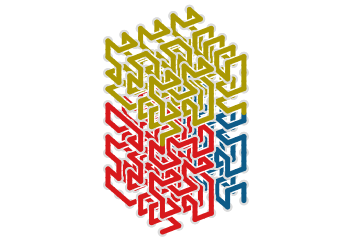
\includegraphics[width=\linewidth]{gilbert3d_eccentric_gamma_example.pdf}
		\label{fig:gilbert3d_eccentric_gamma_example}
		\captionof{figure}{ }
	\end{minipage}

	\begin{minipage}{0.49\textwidth}
		\centering
		\includegraphics[width=\linewidth]{gilbert3d_bulk_template.pdf}
		\label{fig:gilbert3d_bulk_template}
		\captionof{figure}{ }
	\end{minipage}\hfill
	\begin{minipage}{0.49\textwidth}
		\centering
		\includegraphics[width=\linewidth]{gilbert3d_bulk_example.pdf}
		\label{fig:gilbert3d_bulk_example}
		\captionof{figure}{ }
	\end{minipage}

\end{minipage}



\section*{Algorithm}


Algorithm \ref{alg:gilbert2d} and algorithm \ref{alg:gilbert3d} shows the pseudo-code for computing the Gilbert curve in
2D and 3D respectively.
After each subdivision, the origin and local axis are rotated to align with the sub
region and recursively solved.
In the base case where there is a unit length side, a curve in one lower dimension is output (a line for 2D and a 2D Gilbert curve for 3D).
If the width like dimension, $\alpha$, is oblong relative to the height-like dimension, $\beta$,
an eccentric template is used.
For the 3D case, additional checks to see if the remaining side lengths are oblong and, if so, the appropriate eccentric curves are applied.
Otherwise, the bulk recursion is executed.


Note that even in the 2D case, $\alpha$ and $\beta$ are taken to be vectors in 3D.
The generalization to 3D allows the Gilbert2D function to be used unaltered when the
3D Gilbert curve needs to trace out in-plane sub-curves.

The standard Euclidean two norm ($|v| = \sqrt{v_0^2 + v_1^2 + v_2^2}$) is used
but abuses notation by allowing scalar to vector multiplication ($i \in \mathbb{Z}, v \in \mathbb{Z}^3, i \cdot v \to ( i \cdot v_0, i \cdot v_1, i \cdot v_2 )$).
where the context is clear.
The $\delta(\cdot)$ function returns one of the six directional vectors indicating which of
the major signed axis aligned directions the input vector points to ($(\pm1,0,0), (0,\pm1,0),(0,0,\pm1)$).
The $\div(a,b)$ function is used to do integer division, rounding towards zero in the case of a fractional result.
To make things more concise, a convenience function is used,
$(\Delta( \rho_2,\rho ) \overset{\mathrm{def}}{=} \delta(\rho) \textbf{ if } |\rho _ 2| \equiv 1 \bmod{2} \text{ and } |\rho| > 2)$,
that prefers even lengths in the non-degenerate case.

Random access functions to convert from index to position or position to index can be created by modifying the presented algorithms
with short circuit conditionals, bypassing path calculation but keeping a running total of positions that would have been traversed.
Each sub-region is an axis-aligned rectangle or cuboid, allowing for easy calculation of path length as the product of the side lengths for
the given area or volume.

%Algorithm \ref{alg:gilbert3d} shows pseudo-code for computing the 3D Gilbert curve.
%Figures \ref{fig:gilbert3d_eccentric_alpha}, \ref{fig:gilbert3d_eccentric_alpha_example} show the various shape templates
%used to subdivide the region and an example curve with color coded regions.
%As with the \textit{Gilbert2D} function, base cases occur when one dimension is unit length, eccentric templates are used
%for oblong side lengths and the bulk recursion is executed in all other cases.

\section*{Conclusion and Future Directions}

The Gilbert curve presented in this paper provides one interpretation for a generalized Hilbert
curve in 2D and 3D to arbitrary side lengths.
Generalizing a Hilbert space filling curve to arbitrary side lengths is open to interpretation
and the solution presented here is one such adaptation.

When designing an algorithm to generalize the Hilbert curve, four features that might be desirable are:

\begin{table}[h]
  \centering
  \begin{tabular}[t]{l|l}
    \textit{Hilbert-esque} & Reduces to a Hilbert curve when side lengths are equal and are exact powers of two \\
    \textit{Stability} & Curve realizations converge as the cuboid side lengths increase proportionally \\
    \textit{Harmony} & Realizations use eccentric splits to reduce the \textit{defect} \\
    \textit{Notch-Limited} & Curve realizations are notch free or limited to a single notch if necessary \\
  \end{tabular}
\end{table}

The 2D Gilbert curve presented here has all of these properties while the 3D Gilbert curve lacks harmony and the notch-limited feature.

Future work could focus on creating 3D Gilbert curve that has all of these features, perhaps by relaxing strict endpoint requirements
at the cuboid corners.
Some other natural ideas are to extend the concepts above to other space filling curves or circuits,
or, more generally, to try and create an arbitrary space filling curve in a cuboid region with arbitrary endpoints.

A libre/free/open implementation for the Gilbert curve in 2D and 3D has been developed and can be downloaded from its
repository \footnote{ \label{gilbert-url} \url{https://github.com/jakubcerveny/gilbert} }.


{\setlength{\baselineskip}{13pt} % tighten line spacing for bibliography
\raggedright        % no right justification for References
\begin{thebibliography}{99}

  %\bibitem{anders2009} S. Anders. ``Visualization of genomic data with the Hilbert curve.'' \textit{Bioinformatics}, vol.~25, no.~10, pp. ~ 1231-1235, 2009.  \url{https://doi.org/10.1093/bioinformatics/btp152}

  %\bibitem{cortesi2011} A. Cortesi. \textit{Visualizing binaries with space-filling curves}. 2011. \url{https://corte.si/posts/visualisation/binvis/}.

  %\bibitem{sagan1994} H. Sagan. \textit{Space-Filling Curves}, 1994 ed. Springer, 1994.

  \bibitem{lutanho2003} L. Tautenhahn. \textit{Draw a space-filling curve of arbitrary size}, 2003. \url{https://lutanho.net/pic2html/draw_sfc.html}.

  %\bibitem{zhang2006} J. Zhang, S. Kamata, and Y. Ueshige. ``A Pseudo-Hilbert Scan Algorithm for Arbitrarily-Sized Rectangle Region.'' \textit{Advances in Machine Vision, Image Processing, and Pattern Analysis}, Berlin, Heidelberg, 2006, pp. 290-299.






%
%\bibitem{Chang}
%W. Chang. \LaTeX\ \textit{Cheat Sheet}. 2014. \url{http://wch.github.io/latexsheet/}.
%
%\bibitem{EJCx}
%M.\ Chladn\'y and M.\ \v Skoviera. ``Factorisation of Snarks.'' \textit{Electronic Journal
%of Combinatorics}, vol.~17, no.~1, R32, 2010.
%\url{http://www.combinatorics.org/Volume_17/PDF/v17i1r32.pdf}.
%
%\bibitem{Coxeter} H.\ S.\ M.\ Coxeter. ``The Non-Euclidean Symmetry of Escher's Picture
%Circle Limit III.'' \textit{Leonardo}, vol.~12, no.~1, 1979, pp.~19--25.
%
%\bibitem{easychair} EasyChair. Log in page. \url{https://easychair.org/account/signin.cgi}.
%
%\bibitem{Gratzer} G.\ Gr\"atzer. \textit{More Math Into} \LaTeX, 4th ed. Springer, 2007.
%
%\bibitem{Sequin2016} C.\ H.\ S\'equin. ``From Klein Bottles to Modular Super-Bottles.''
%\textit{Bridges Conference Proceedings}, Jyv\"askyl\"a, Finland, Aug. 9--13,
%2016, pp.~41--48. \url{http://archive.bridgesmathart.org/2016/bridges2016-41.html}.
%

\end{thebibliography}
} % end setlength, raggedright

%\begin{figure}[ht]
%  \centering
%  %{\transparent{0.4}\includegraphics[width=\linewidth]{gilbert_bd50x10.pdf}}
%  \includegraphics[width=\linewidth]{gilbert_bd50x10.pdf}
%  \label{fig:footerGilbert}
%\end{figure}

\end{document}


